%! TEX program = xelatex
%! TEX root = ../root.tex

\section{实验原理}
\subsection{CSR指令}
实现RSIC-V的中断与异常首先就需要能够对CSR进行读写操作,M特权模式提供了如下六种指令进行操作。\\

\begin{figure}[H] %H为当前位置,!htb为忽略美学标准,htbp为浮动图形
    \centering %图片居中
    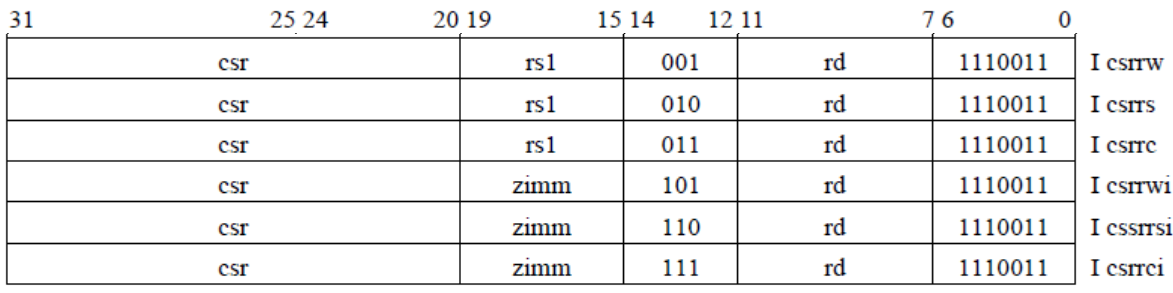
\includegraphics[width=1.0\textwidth]{figs/csr.png} %插入图片,[]中设置图片大小,{}中是图片文件名
    \caption{CSR指令} %最终文档中希望显示的图片标题
    \label{Fig.1} %用于文内引用的标签
\end{figure}

介绍完指令格式之后,CSR每个指令的作用如下\\

\begin{tabular}{|l|c|r|}
    \hline
    操作名 & 使用方式 & 操作方式\\
    \hline
    csrrw & csrrw rd, csr, rs1 & t = CSRs[csr]; CSRs[csr] = x[rs1]; x[rd] = t \\
    \hline
    csrrs & csrrs rd, csr, rs1 & t = CSRs[csr]; CSRs[csr] = t | x[rs1]; x[rd] = t \\
    \hline
    csrrc & csrrc rd, csr, rs1  & t = CSRs[csr]; CSRs[csr] = t \& ~x[rs1]; x[rd] = t \\
    \hline
    jump I-type & 1100111 & jalr \\
    \hline
    S-type & 0100011 & sw \\
    \hline 
    B-type & 1100011 & beq, bne, blt, bge, bltu, bgeu \\
    \hline
    U-type(lui) & 0110111 & lui \\
    \hline
    U-type(auipc) & 0010111 & auipc \\
    \hline
    J-type & 1101111 & jal \\
    \hline
\end{tabular} \\

根据指令格式,我们可以从中知道立即数的存储方式:\\

% \begin{tabular}{|r|l|}
%     \hline
%     操作类型 & 立即数组织方式 \\
%     \hline 
%     I-type & Imm = \{ {21\{Ins[31]}\}, Ins[30:25], Ins[24:21], Ins[20] \} \\
%     \hline
%     S-type & Imm = \{ \{21\{Ins[31]\}\}, Ins[30:25], Ins[11:8], Ins[7] \} \\
%     \hline
%     U-type & Imm = \{ Ins[31], Ins[30:20], Ins[19:12], 12'b0 \} \\
%     \hline
%     J-type & Imm = \{ \{12\{Ins[31]\}\}, Ins[19:12], Ins[20], Ins[30:25], Ins[24:21], 1'b0 \} \\
%     \hline
%     B-type & Imm = \{ \{20\{Ins[31]\}\}, Ins[7], Ins[30:25], Ins[11:8], 1'b0\} \\
%     \hline
% \end{tabular} \\

% 需要注意的是,之所以U-type、J-type、B-type指令的立即数需要末尾加0,与PC地址恒为2的倍数有关,省略恒为0的最末尾可以使得立即数表示大一倍,可能我们会注意到PC地址
% 实际上恒为4的倍数,为什么不直接省略末尾两个0呢?是因为还有一种2Byte的压缩指令,如果省略两位,那它将无法表示。

% \subsection{Control Unit}
% 本实验中,ControlUnit复杂产生指令的控制信号、ALU的操作信号与比较器的操作信号
% 在此部分仅说明需要填充的内容,首先是用于判断跳转指令类型的信号,根据指令类型(OpCode)与funct3判断其类型。

% \begin{tabular}{|r|c|c|c|c|l|}
%     \hline
%     funct3 & 跳转指令类型 & Load类型 & Store类型 \\
%     \hline 
%     3'b000 & BEQ & LB &  SB \\
%     \hline
%     3'b001 & BNE & LH & SH \\
%     \hline
%     3'b010 & - & LW & SW \\
%     \hline
%     3'b100 & BLT & LBU & - \\
%     \hline
%     3'b101 & BGE & LHU & - \\
%     \hline
%     3'b110 & BLTU & - & - \\
%     \hline
%     3'b111 & BGEU & - & - \\
%     \hline
% \end{tabular} \\

% 信号LUI, AUIPC, JAL与JALR只需判断输入OpCode是否等于对应OpCode即可。而Branch跳转控制信号则是JAL, JALR与Branch是否跳转信号(Branch \& cmp\_res)的或运算,比较器的控制信号直接将输入的funct3传入即可。 \\
% 比较重要的是ALU的两个输入口的操作数选择信号,A口选择器有两个输入:PC值(0)与rs1\_data(1),根据指令操作方式我们可以判断出只有AUIPC, JAL与JALR需要在EXE阶段对PC值进行运算,所以它们的控制信号应该置0,其他指令均置1;
% B口选择器也有两个输入rs2\_data与立即数,根据指令操作方式我们判断出I类型指令,Load类型指令,Store类型指令,LUI与AUIPC均需要在EXE阶段利用立即数进行计算。 \\
% rs1use与rs2use分别是寄存器的rs1与rs2是否被使用的信号,根据前述指令类型我们可以比较容易的得到结果。 \\
% 最后是hazard\_optype信号,此信号用于传递给HazardUnit以便识别当前指令的类型,这个信号的使用可以减少很多信号的传递。

% \begin{lstlisting}[language = {verilog}]
% module CtrlUnit(
%     input[31:0] inst,
%     input cmp_res,
%     output Branch, ALUSrc_A, ALUSrc_B, DatatoReg, RegWrite, mem_w,
%         MIO, rs1use, rs2use,
%     output [1:0] hazard_optype,
%     output [2:0] ImmSel, cmp_ctrl,
%     output [3:0] ALUControl,
%     output JALR
% );

%     //跳转指令的类型判断信号
%     wire BEQ = Bop & funct3_0;                    //to fill sth. in 
%     wire BNE = Bop & funct3_1;                    //to fill sth. in 
%     wire BLT = Bop & funct3_4;                    //to fill sth. in 
%     wire BGE = Bop & funct3_5;                    //to fill sth. in 
%     wire BLTU = Bop & funct3_6;                   //to fill sth. in 
%     wire BGEU = Bop & funct3_7;                   //to fill sth. in 
%     //Load指令的类型判断
%     wire LB = Lop & funct3_0;                     //to fill sth. in 
%     wire LH = Lop & funct3_1;                     //to fill sth. in 
%     wire LW = Lop & funct3_2;                     //to fill sth. in 
%     wire LBU =Lop & funct3_4;                     //to fill sth. in 
%     wire LHU =Lop & funct3_5;                     //to fill sth. in 
%     //Store指令的类型判断
%     wire SB = Sop & funct3_0;                     //to fill sth. in 
%     wire SH = Sop & funct3_1;                     //to fill sth. in 
%     wire SW = Sop & funct3_2;                     //to fill sth. in 
    
%     wire LUI   = opcode == 7'b0110111;            //to fill sth. in 
%     wire AUIPC = opcode == 7'b0010111;            //to fill sth. in 

%     wire JAL  = opcode == 7'b1101111;              //to fill sth. in 
%     assign JALR = opcode == 7'b1100111;            //to fill sth. in 
%     //跳转总控制信号
%     assign Branch = (cmp_res & B_valid) | JAL | JALR;   //to fill sth. in 
%     //比较器控制信号
%     assign cmp_ctrl = funct3;                           //to fill sth. in 
%     //ALU的A操作数选择信号
%     assign ALUSrc_A = (AUIPC | JAL | JALR) ? 0 : 1;           //to fill sth. in 
%     //ALU的B操作数选择信号
%     assign ALUSrc_B = (I_valid | L_valid | S_valid | LUI | AUIPC)? 1 : 0;   //to fill sth. in 

%     assign rs1use = R_valid|S_valid|B_valid|L_valid|I_valid;         //to fill sth. in 

%     assign rs2use = R_valid|S_valid|B_valid;                         //to fill sth. in 

%     assign hazard_optype = (R_valid | I_valid | LUI | AUIPC | JAL | JALR) ? 2'b00:
%                             S_valid ? 2'b01:
%                             L_valid ? 2'b10:2'b11;                  //to fill sth. in 

% endmodule
% \end{lstlisting}

% \subsection{Comperator}
% 比较器是根据输入控制信号(ctrl)进行相应的比较操作并将结果输出,
% 比较器的操作比较简单,就是将对应比较操作的结果输出即可,默认为0

% \begin{lstlisting}[language = {verilog}]
% module cmp_32(  input [31:0] a,
%                 input [31:0] b,
%                 input [2:0] ctrl,
%                 output c
%     );

%     //to fill sth. in ()
%     assign c =  EQ  ? res_EQ  : 
%                 NE  ? res_NE  : 
%                 LT  ? res_LT  : 
%                 LTU ? res_LTU :
%                 GE  ? res_GE  :
%                 GEU ? res_GEU :
%                       0;          

% endmodule
% \end{lstlisting}

% \subparagraph{}

% \subsection{数据通路}
% 完成了个部件的设计,数据通路就是将各个部分连接起来,保证各功能正常实现的关键部分,下面是总体的原理图

% \begin{figure}[H] %H为当前位置,!htb为忽略美学标准,htbp为浮动图形
%     \centering %图片居中
%     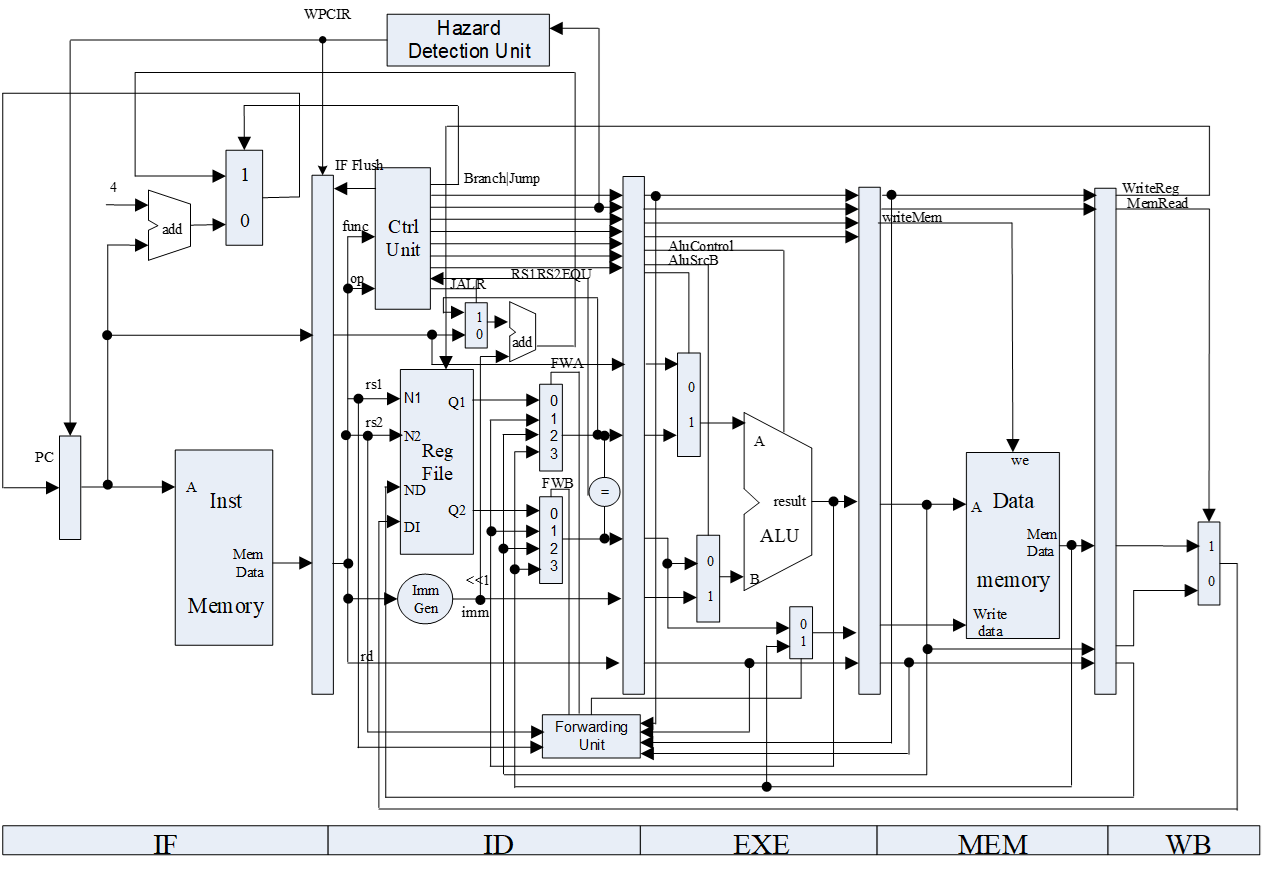
\includegraphics[width=1.0\textwidth]{DataPath.png} %插入图片,[]中设置图片大小,{}中是图片文件名
%     \caption{Datapath} %最终文档中希望显示的图片标题
%     \label{Fig.2} %用于文内引用的标签
% \end{figure}

% 数据通路的补充就是根据原理图连线即可,具体的源代码如下
% \begin{lstlisting}[language = {verilog}]
% module  RV32core(
%         input debug_en,  // debug enable
%         input debug_step,  // debug step clock
%         input [6:0] debug_addr,  // debug address
%         output[31:0] debug_data,  // debug data
%         input clk,  // main clock
%         input rst,  // synchronous reset
%         input interrupter  // interrupt source, for future use
%     );

%     wire debug_clk;

%     debug_clk clock(.clk(clk),.debug_en(debug_en),.debug_step(debug_step),.debug_clk(debug_clk));

%     wire Branch_ctrl, JALR, RegWrite_ctrl, mem_w_ctrl, MIO_ctrl,
%         ALUSrc_A_ctrl, ALUSrc_B_ctrl, DatatoReg_ctrl, rs1use_ctrl, rs2use_ctrl;
%     wire[1:0] hazard_optype_ctrl;
%     wire[2:0] ImmSel_ctrl, cmp_ctrl;
%     wire[3:0] ALUControl_ctrl;

%     wire forward_ctrl_ls;
%     wire[1:0] forward_ctrl_A, forward_ctrl_B;

%     wire PC_EN_IF;
%     wire [31:0] PC_IF, next_PC_IF, PC_4_IF, inst_IF;

%     wire reg_FD_EN,reg_FD_stall,reg_FD_flush, cmp_res_ID;
%     wire [31:0] jump_PC_ID, PC_ID, inst_ID, Debug_regs, rs1_data_reg, rs2_data_reg,
%         Imm_out_ID, rs1_data_ID, rs2_data_ID, addA_ID;
    
%     wire reg_DE_EN, reg_DE_flush, RegWrite_EXE, mem_w_EXE, MIO_EXE,
%         ALUSrc_A_EXE, ALUSrc_B_EXE, ALUzero_EXE, ALUoverflow_EXE, DatatoReg_EXE;
%     wire[2:0] u_b_h_w_EXE;
%     wire[3:0] ALUControl_EXE;
%     wire[4:0] rs1_EXE, rs2_EXE, rd_EXE;
%     wire[31:0] ALUout_EXE, PC_EXE, inst_EXE, rs1_data_EXE, rs2_data_EXE, Imm_EXE,
%         ALUA_EXE, ALUB_EXE, Dataout_EXE;
    
%     wire reg_EM_EN, reg_EM_flush, RegWrite_MEM, DatatoReg_MEM, mem_w_MEM, MIO_MEM;
%     wire[2:0] u_b_h_w_MEM;
%     wire[4:0] rd_MEM;
%     wire[31:0] ALUout_MEM, PC_MEM, inst_MEM, Dataout_MEM, Datain_MEM;


%     wire reg_MW_EN, RegWrite_WB, DatatoReg_WB;
%     wire[4:0] rd_WB;
%     wire [31:0] wt_data_WB, PC_WB, inst_WB, ALUout_WB, Datain_WB;


%     // IF
%     REG32 REG_PC(.clk(debug_clk),.rst(rst),.CE(PC_EN_IF),.D(next_PC_IF),.Q(PC_IF));
    
%     add_32 add_IF(.a(PC_IF),.b(32'd4),.c(PC_4_IF));

%     //to fill sth. in ()
%     MUX2T1_32 mux_IF(.I0(PC_4_IF),.I1(jump_PC_ID),.s(Branch_ctrl),.o(next_PC_IF));        

%     ROM_D inst_rom(.a(PC_IF[8:2]),.spo(inst_IF));


%     // ID
%     REG_IF_ID reg_IF_ID(.clk(debug_clk),.rst(rst),.EN(reg_FD_EN),.Data_stall(reg_FD_stall),
%         .flush(reg_FD_flush),.PCOUT(PC_IF),.IR(inst_IF),

%         .IR_ID(inst_ID),.PCurrent_ID(PC_ID));
    
%     CtrlUnit ctrl(.inst(inst_ID),.cmp_res(cmp_res_ID),.Branch(Branch_ctrl),.ALUSrc_A(ALUSrc_A_ctrl),
%         .ALUSrc_B(ALUSrc_B_ctrl),.DatatoReg(DatatoReg_ctrl),.RegWrite(RegWrite_ctrl),
%         .mem_w(mem_w_ctrl),.MIO(MIO_ctrl),.rs1use(rs1use_ctrl),.rs2use(rs2use_ctrl),
%         .hazard_optype(hazard_optype_ctrl),.ImmSel(ImmSel_ctrl),.cmp_ctrl(cmp_ctrl),
%         .ALUControl(ALUControl_ctrl),.JALR(JALR));
    
%     Regs register(.clk(debug_clk),.rst(rst),.L_S(RegWrite_WB),.R_addr_A(inst_ID[19:15]),
%         .R_addr_B(inst_ID[24:20]),.rdata_A(rs1_data_reg),.rdata_B(rs2_data_reg),
%         .Wt_addr(rd_WB),.Wt_data(wt_data_WB),
%         .Debug_addr(debug_addr[4:0]),.Debug_regs(Debug_regs));
    
%     ImmGen imm_gen(.ImmSel(ImmSel_ctrl),.inst_field(inst_ID),.Imm_out(Imm_out_ID));
    
%     //to fill sth. in ()
%     MUX4T1_32 mux_forward_A(.I0(rs1_data_reg),.I1(ALUout_EXE),.I2(ALUout_MEM),.I3(Datain_MEM),        
%         .s(forward_ctrl_A),.o(rs1_data_ID));
    
%     //to fill sth. in ()
%     MUX4T1_32 mux_forward_B(.I0(rs2_data_reg),.I1(ALUout_EXE),.I2(ALUout_MEM),.I3(Datain_MEM),        
%         .s(forward_ctrl_B),.o(rs2_data_ID));
    
%     MUX2T1_32 mux_branch_ID(.I0(PC_ID),.I1(rs1_data_ID),.s(JALR),.o(addA_ID));

%     add_32 add_branch_ID(.a(addA_ID),.b(Imm_out_ID),.c(jump_PC_ID));

%     cmp_32 cmp_ID(.a(rs1_data_ID),.b(rs2_data_ID),.ctrl(cmp_ctrl),.c(cmp_res_ID));        
    
%     HazardDetectionUnit hazard_unit(.clk(debug_clk),.Branch_ID(Branch_ctrl),.rs1use_ID(rs1use_ctrl),
%         .rs2use_ID(rs2use_ctrl),.hazard_optype_ID(hazard_optype_ctrl),.rd_EXE(rd_EXE),
%         .rd_MEM(rd_MEM),.rs1_ID(inst_ID[19:15]),.rs2_ID(inst_ID[24:20]),.rs2_EXE(rs2_EXE),
%         .PC_EN_IF(PC_EN_IF),.reg_FD_EN(reg_FD_EN),.reg_FD_stall(reg_FD_stall),
%         .reg_FD_flush(reg_FD_flush),.reg_DE_EN(reg_DE_EN),.reg_DE_flush(reg_DE_flush),
%         .reg_EM_EN(reg_EM_EN),.reg_EM_flush(reg_EM_flush),.reg_MW_EN(reg_MW_EN),
%         .forward_ctrl_ls(forward_ctrl_ls),.forward_ctrl_A(forward_ctrl_A),
%         .forward_ctrl_B(forward_ctrl_B));

%     // EX
%     REG_ID_EX reg_ID_EX(.clk(debug_clk),.rst(rst),.EN(reg_DE_EN),.flush(reg_DE_flush),.IR_ID(inst_ID),
%         .PCurrent_ID(PC_ID),.rs1_addr(inst_ID[19:15]),.rs2_addr(inst_ID[24:20]),.rs1_data(rs1_data_ID),
%         .rs2_data(rs2_data_ID),.Imm32(Imm_out_ID),.rd_addr(inst_ID[11:7]),.ALUSrc_A(ALUSrc_A_ctrl),
%         .ALUSrc_B(ALUSrc_B_ctrl),.ALUC(ALUControl_ctrl),.DatatoReg(DatatoReg_ctrl),
%         .RegWrite(RegWrite_ctrl),.WR(mem_w_ctrl),.u_b_h_w(inst_ID[14:12]),.MIO(MIO_ctrl),

%         .PCurrent_EX(PC_EXE),.IR_EX(inst_EXE),.rs1_EX(rs1_EXE),.rs2_EX(rs2_EXE),
%         .A_EX(rs1_data_EXE),.B_EX(rs2_data_EXE),.Imm32_EX(Imm_EXE),.rd_EX(rd_EXE),
%         .ALUSrc_A_EX(ALUSrc_A_EXE),.ALUSrc_B_EX(ALUSrc_B_EXE),.ALUC_EX(ALUControl_EXE),
%         .DatatoReg_EX(DatatoReg_EXE),.RegWrite_EX(RegWrite_EXE),.WR_EX(mem_w_EXE),
%         .u_b_h_w_EX(u_b_h_w_EXE),.MIO_EX(MIO_EXE));
    
%     //to fill sth. in ()
%     MUX2T1_32 mux_A_EXE(.I0(PC_EXE),.I1(rs1_data_EXE),.s(ALUSrc_A_EXE),.o(ALUA_EXE));  
%     //to fill sth. in ()   
%     MUX2T1_32 mux_B_EXE(.I0(rs2_data_EXE),.I1(Imm_EXE),.s(ALUSrc_B_EXE),.o(ALUB_EXE));       

%     ALU alu(.A(ALUA_EXE),.B(ALUB_EXE),.Control(ALUControl_EXE),
%         .res(ALUout_EXE),.zero(ALUzero_EXE),.overflow(ALUoverflow_EXE));
    
%     //to fill sth. in ()
%     MUX2T1_32 mux_forward_EXE(.I0(rs2_data_EXE),.I1(Datain_MEM),.s(forward_ctrl_ls),.o(Dataout_EXE));        


%     // MEM
%     REG_EX_MEM reg_EXE_MEM(.clk(debug_clk),.rst(rst),.EN(reg_EM_EN),.flush(reg_EM_flush),
%         .IR_EX(inst_EXE),.PCurrent_EX(PC_EXE),.ALUO_EX(ALUout_EXE),.B_EX(Dataout_EXE),
%         .rd_EX(rd_EXE),.DatatoReg_EX(DatatoReg_EXE),.RegWrite_EX(RegWrite_EXE),
%         .WR_EX(mem_w_EXE),.u_b_h_w_EX(u_b_h_w_EXE),.MIO_EX(MIO_EXE),

%         .PCurrent_MEM(PC_MEM),.IR_MEM(inst_MEM),.ALUO_MEM(ALUout_MEM),.Datao_MEM(Dataout_MEM),
%         .rd_MEM(rd_MEM),.DatatoReg_MEM(DatatoReg_MEM),.RegWrite_MEM(RegWrite_MEM),
%         .WR_MEM(mem_w_MEM),.u_b_h_w_MEM(u_b_h_w_MEM),.MIO_MEM(MIO_MEM));
    
%     RAM_B data_ram(.addra(ALUout_MEM),.clka(debug_clk),.dina(Dataout_MEM), 
%         .wea(mem_w_MEM),.douta(Datain_MEM),.mem_u_b_h_w(u_b_h_w_MEM));


%     // WB
%     REG_MEM_WB reg_MEM_WB(.clk(debug_clk),.rst(rst),.EN(reg_MW_EN),.IR_MEM(inst_MEM),
%         .PCurrent_MEM(PC_MEM),.ALUO_MEM(ALUout_MEM),.Datai(Datain_MEM),.rd_MEM(rd_MEM),
%         .DatatoReg_MEM(DatatoReg_MEM),.RegWrite_MEM(RegWrite_MEM),

%         .PCurrent_WB(PC_WB),.IR_WB(inst_WB),.ALUO_WB(ALUout_WB),.MDR_WB(Datain_WB),
%         .rd_WB(rd_WB),.DatatoReg_WB(DatatoReg_WB),.RegWrite_WB(RegWrite_WB));
    
%     MUX2T1_32 mux_WB(.I0(ALUout_WB),.I1(Datain_WB),.s(DatatoReg_WB),.o(wt_data_WB));


%     wire [31:0] Test_signal;
%     assign debug_data = debug_addr[5] ? Test_signal : Debug_regs;
    
%     CPUTEST    U1_3(.PC_IF(PC_IF),
%                     .PC_ID(PC_ID),
%                     .PC_EXE(PC_EXE),
%                     .PC_MEM(PC_MEM),
%                     .PC_WB(PC_WB),
%                     .PC_next_IF(next_PC_IF),
%                     .PCJump(jump_PC_ID),
%                     .inst_IF(inst_IF),
%                     .inst_ID(inst_ID),
%                     .inst_EXE(inst_EXE),
%                     .inst_MEM(inst_MEM),
%                     .inst_WB(inst_WB),
%                     .PCEN(PC_EN_IF),
%                     .Branch(Branch_ctrl),
%                     .PCSource(Branch_ctrl),
%                     .RS1DATA(rs1_data_reg),
%                     .RS2DATA(rs2_data_reg),
%                     .Imm32(Imm_out_ID),
%                     .ImmSel(ImmSel_ctrl),
%                     .ALUC(ALUControl_ctrl),
%                     .ALUSrc_A(ALUSrc_A_ctrl),
%                     .ALUSrc_B(ALUSrc_B_ctrl),
%                     .A(ALUA_EXE),
%                     .B(ALUB_EXE),
%                     .ALU_out(ALUout_MEM),
%                     .Datai(Datain_MEM),
%                     .Datao(Dataout_MEM),
%                     .Addr(Addr),
%                     .WR(MWR),
%                     .MIO(MIO_MEM),
%                     .WDATA(wt_data_WB),
%                     .DatatoReg(DatatoReg_WB),
%                     .RegWrite(RegWrite_WB),
%                     .data_hazard(reg_FD_stall),
%                     .control_hazard(Branch_ctrl),

%                     .Debug_addr(debug_addr[4:0]),
%                     .Test_signal(Test_signal)    
%                     );

% endmodule
% \end{lstlisting}

% \subsection{HazardUnit}
% 在此次的实验中,Hazard由结构竞争、数据冒险和控制竞争三部分组成,出于效率与实现复杂度的考虑
% 本模块被设计在ID阶段,利用段寄存的Flush与Stall功能实现插入bubble或者清空段寄存器数据
% 并且本次实验还设计了Forward Units以减少停顿次数,提高流水线效率,同时本模块中实现了Predict-Not-Taken的
% 跳转策略,在ID阶段识别并执行跳转语句。具体的设计分几部分阐述如下:

% \subparagraph{ForwardUnits}
% 前送只涉及到EX, MEM, WB三个阶段的数据前送,在此实验中分为ALU的两个数据输入口进行讨论,
% 其中ALU的1号操作数口接受来自:
% \begin{itemize}
%     \item [1.] ID阶段读取的寄存器值的rs1\_val
%     \item [2.] EXE阶段的上一条指令EX阶段的ALU计算结果
%     \item [3.] MEM阶段的上一条指令EX阶段的ALU计算结果
%     \item [4.] WB阶段将要写回Memory的数据结果
% \end{itemize}
% 当没有前递时,直接选择ID阶段读取的寄存器值,但只涉及到两条运算指令的RAW并且EX阶段运算得到的结果在ID阶段就需要使用时选择2号数据,当两条产生冲突的普通运算指令
% 中间隔了一条无关指令,也即MEM阶段还未写入的数据在ID阶段又需要使用时选择3号数据,4号数据是提供给涉及到Load与一条普通运算指令之间产生的数据冲突使用的,也即当Load指令
% 所对应的内存数据还未写入寄存器但ID阶段又使用到此寄存器时选择数据4。 \\
% 所以前送ALU操作数1口的条件应该是:
% \begin{itemize}
%     \item [1.] regw\_exe \& rs1\_ID==rd\_EXE \& rs1use\_ID
%     \item [2.] regw\_mem \& rs1\_ID==rd\_MEM \& rs1use\_ID \& ~mem\_load
%     \item [3.] regw\_mem \& rs1\_ID==rd\_MEM \& rs1use\_ID \& mem\_load
%     \item [4.] others
% \end{itemize}
% ALU操作数的2口分析与1口类似,ALU的2号操作数口接受来自:
% \begin{itemize}
%     \item [1.] ID阶段读取的寄存器值的rs2\_val
%     \item [2.] EXE阶段的上一条指令EX阶段的ALU计算结果
%     \item [3.] MEM阶段的上一条指令EX阶段的ALU计算结果
%     \item [4.] WB阶段将要写回Memory的数据结果
% \end{itemize}
% 前送ALU操作数2口的条件应该是:
% \begin{itemize}
%     \item [1.] regw\_exe \& rs2\_ID==rd\_EXE \& rs2use\_ID
%     \item [2.] regw\_mem \& rs2\_ID==rd\_MEM \& rs2use\_ID \& ~mem\_load
%     \item [3.] regw\_mem \& rs2\_ID==rd\_MEM \& rs2use\_ID \& mem\_load
%     \item [4.] others
% \end{itemize}
% 这样使得涉及到算数指令的Read After Write冲突无需任何停顿即可得到正确结果,使得涉及到Load指令的RAW情形仅需一次停顿即可避免数据冲突。 \\
% 除了ALU的前递之外,此次实验还存在一种特殊的前递,Load指令之后紧接Store指令并发生冲突时,需要通过ls信号控制将Load阶段将要写入内存的寄存器值前递给Store指令。
% \subparagraph{Predict-Not-Taken}
% 对于跳转指令的判断,我组均是在ID阶段判断并跳转,若ID阶段检测到不满足跳转条件(Branch指令不跳转且不为JAL, JALR指令),
% 则流水线继续执行,若ID阶段检测到跳转(Branch满足跳转条件或Jal, Jalr必定跳转),则将下一条PC地址的值修改为跳转的目标地址,并且将IF/ID段寄存器的值
% Flush掉(清空),这样可以使得无效指令全部被清空,并且跳转指令的剩下部分继续向后流动直至执行完毕(例如jal, jalr指令还需将PC + 4的值写入寄存器)
% 所以此实验实现了只Flush一个段寄存器无需Stall的Predict-Not-Taken策略

% \subparagraph{DataHazard}
% 尽管拥有了前递单元,实验中仅需将涉及到Load指令的RAW情形还是无法仅通过前递解决,也就是说Load与后续一条季运算指令的数据冲突需要使得后续指令停顿一拍,在EX阶段判断并插入bubble,
% 并且插入bubble的方式就是将EX/MEM段寄存器Flush掉,并使得IF/ID与ID/EX段寄存器Stall(停顿)一个周期 \\

% 综上原理,我组设计的HazardUnit代码如下:
% \begin{lstlisting}[language = {verilog}]
% `timescale 1ps/1ps

% module HazardDetectionUnit(
%     input clk,
%     input Branch_ID, rs1use_ID, rs2use_ID,
%     input[1:0] hazard_optype_ID,
%     input[4:0] rd_EXE, rd_MEM, rs1_ID, rs2_ID, rs2_EXE,
%     output PC_EN_IF, reg_FD_EN, reg_FD_stall, reg_FD_flush,
%         reg_DE_EN, reg_DE_flush, reg_EM_EN, reg_EM_flush, reg_MW_EN,
%     output forward_ctrl_ls,
%     output[1:0] forward_ctrl_A, forward_ctrl_B
% );
%     wire regw_exe, regw_mem;
%     reg [1:0] hazard_optype_EXE;
%     reg [1:0] hazard_optype_MEM;
%     always@(posedge clk) begin
%         hazard_optype_MEM=hazard_optype_EXE;
%         hazard_optype_EXE=hazard_optype_ID;
%     end
%     wire id_store=hazard_optype_ID==2'b01 ? 1:0;
%     wire exe_load=hazard_optype_EXE==2'b10 ? 1:0;
%     wire mem_load=hazard_optype_MEM==2'b10 ? 1:0;
%     wire exe_store=hazard_optype_EXE==7'b01 ? 1:0;
%     wire mem_store=hazard_optype_MEM==7'b01 ? 1:0;
%     assign regw_exe=(hazard_optype_EXE==2'b00) || (hazard_optype_EXE==2'b10);
%     assign regw_mem=(hazard_optype_MEM==2'b00) || (hazard_optype_MEM==2'b10);
%     wire stall=exe_load && !id_store && ((rs1_ID==rd_EXE && rs1use_ID) || (rs2_ID==rd_EXE && rs2use_ID));
    
%     assign forward_ctrl_A=(regw_exe && rs1_ID==rd_EXE && rs1use_ID)? 2'b01:
%                             (regw_mem && rs1_ID==rd_MEM && rs1use_ID)? (mem_load ? 2'b11:2'b10):2'b00;
%     assign forward_ctrl_B=(regw_exe && rs2_ID==rd_EXE && rs2use_ID)? 2'b01:
%                             (regw_mem && rs2_ID==rd_MEM && rs2use_ID)? (mem_load ? 2'b11:2'b10):2'b00;
%     assign forward_ctrl_ls=(rs2_EXE==rd_MEM && mem_load && exe_store)?1:0;
    
%     assign PC_EN_IF=!stall;
%     assign reg_FD_EN=1;
%     assign reg_FD_stall=stall;
%     assign reg_FD_flush=Branch_ID;
%     assign reg_DE_EN=1;
%     assign reg_DE_flush=stall;
%     assign reg_EM_EN=1;
%     assign reg_EM_flush=stall;
%     assign reg_MW_EN=1;

% endmodule    
% \end{lstlisting}